\chapter{Acceptance Test}\label{ch:Tests}
In this chapter the delimited requirements will be tested. First the test site will be presented by a plan view and a table of objects from the test site.

\section{Test site}
The test site consist of the obstacles stated in table \ref{tab:obstacles}. Pictures of the test site can be found in Appendix A.

\begin{table} [h]
    \centering
    \begin{tabu} to 1\textwidth { | X[c] | X[c] | X[c] | }
     \hline
     Obstacles & \multicolumn{2}{c|}{Size} \\
     \hline
     Football table & Length 145 cm & Width 75 cm \\
     \hline
     Bench & Length 200 cm & Width 40 cm \\
     \hline
     Carpet & Length 200 cm & Width 115 cm \\
     \hline
     Small pot & Length 35 cm & Width 35 cm \\
     \hline
     Big pot & Length 95 cm & Width 40 cm \\
     \hline
     Upper staircase & Length 180 cm & Width 115 cm \\
     \hline
     Lower staircase & Length 600 cm & Depth 18 cm \\
     \hline
     Beer can & Height 16 cm & Diameter 6 cm \\
     \hline
     Wooden pole & Height 41 cm & Width 9 cm\\
     \hline 
    \end{tabu}
    \caption{Table of the sizes of all obstacles from the test site}
    \label{tab:obstacles}
\end{table}
\begin{figure}[h]
    \centering
    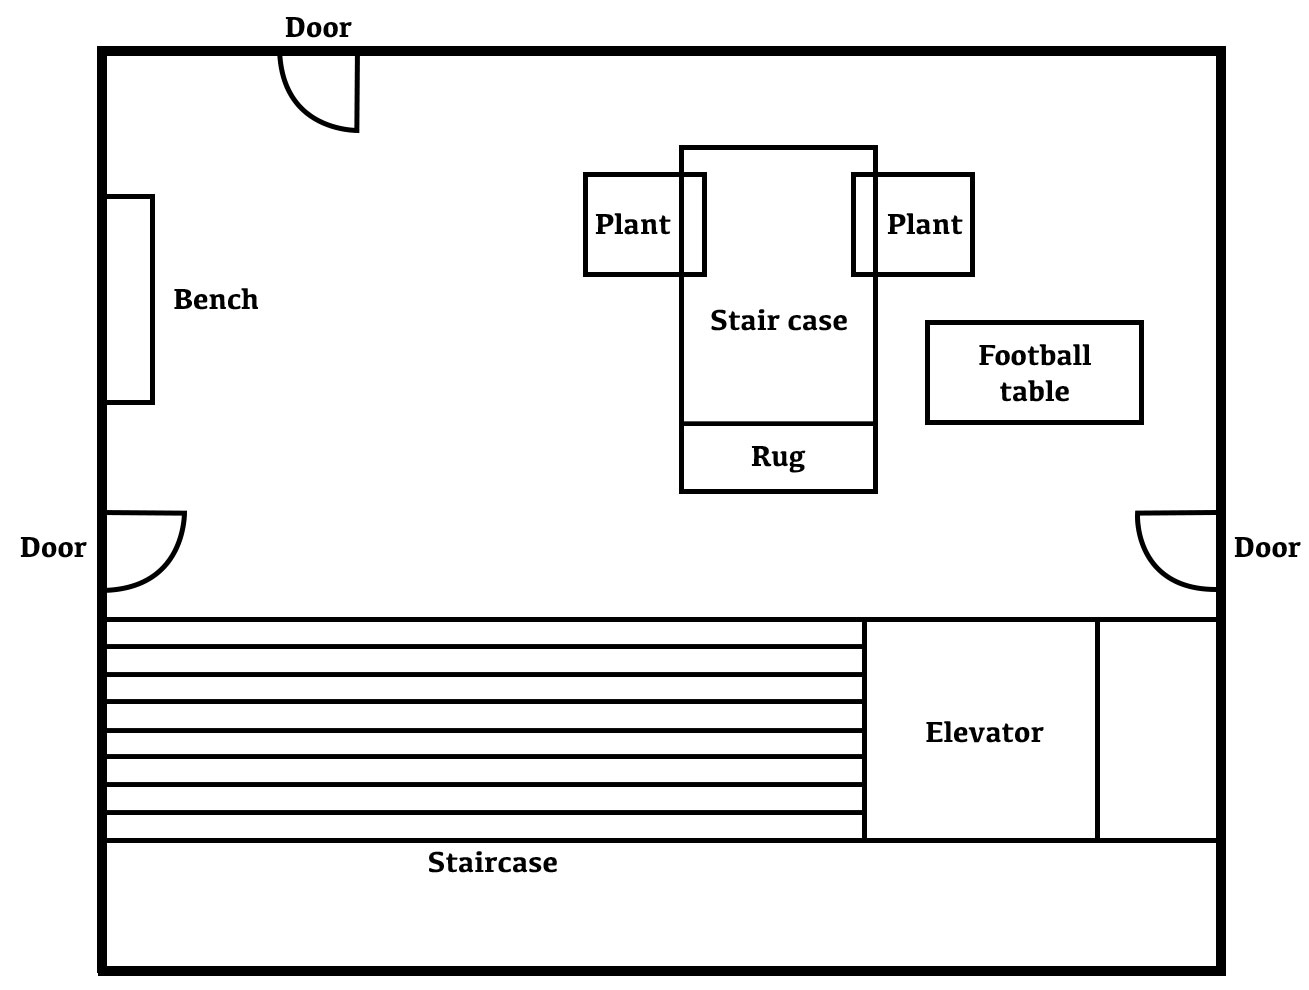
\includegraphics[width=\textwidth]{figures/plantegning.jpg}
    \caption{Test site layout} 
    \label{fig:layout} 
\end{figure}
\newpage

%
%
% Test 1
%
%

\section{Test 1}
The requirement, "The robot has to be able to drive with a distance of 8 m from the router without dropping the connection", is tested by placing the turtlebot near the router's position and drive it 8 m in the opposite direction.\\ 
\newline
First the host computer gets the following commands:

1. \texttt{roscore}

2. \texttt{roslaunch\_bringup minimal.launch}\\
Then the user computer gets the following commands:

1. \texttt{roslaunch turtlebot\_teleop keyboard\_teleop.launch}\\
The user computer should now be able to control the turtlebot.\\
The robot was steered with \texttt{Roslaunch turtlebot\_teleop keyboard\_teleop.launch} from the computer, where the keyboard was used to control the robot.\\
The robot would then move accordingly to the keys 'J', 'L', 'I', ',' and 'K'.\\
\newline
\textbf{Controls:}
\begin{minipage}[t]{.5\textwidth}
\begin{itemize}
    \item J for turning left
    \item L for turning right
    \item I for forward
\end{itemize}
\end{minipage}
\begin{minipage}[t]{.5\textwidth}
    \begin{itemize}
    \item , for backwards
    \item K for stopping
    \end{itemize}
\end{minipage}

\subsection{Result}
The robot drove 8 m without dropping the connection.\\
Test 1 was a success and met the standards of the requirement.

%
%
% Test 2
%
%

\section{Test 2}
The frontier\_exploration node is tested by making a 5x5 m map for the turtlebot to explore.\\
\newline
The host computer got the commands:

1. \texttt{roscore} 

2. \texttt{roslaunch turtlebot\_bringup minimal.launch}

3. \texttt{roslaunch turtlebot\_navigation gmapping\_demo.launch}\\
The user computer was given the commands in two different terminals:

1. \texttt{roslaunch turtlebot\_rviz\_launchers view\_navigation.launch}

2. \texttt{roslaunch turtlebot\_samples exploration.launch}\\
Here it should be possible to make a polygon area in Rviz by using publishing points, which the robot will explore.

\subsection{Result}
The robot explored the 5x5 m map.\\
Test 2 was a success and met the standards of the requirement.

%
%
% Test 3
%
%

\section{Test 3}
The requirement, "It has to be able to move 5 m in 1 min", is tested.\\ 
\newline
First the host computer gets the following commands:

1. \texttt{roscore}

2. \texttt{roslaunch\_bringup minimal.launch}\\
Then the user computer gets the following commands:

1. \texttt{roslaunch turtlebot\_teleop keyboard\_teleop.launch}\\
The user computer should now be able to control the turtlebot.\\
The same procedure is done in this test as in test 1.


\subsection{Result}
The turtlebot moved 5 m in a straight line with the time of 0.28 seconds.\\
Test 3 was successful and met the standards of the requirement. 

%
%
% Test 4
%
%

\section{Test 4}
The requirement, "It has to be able to turn 360${^\circ}$ in under a minute", is tested.\\ 
The same procedure is done in this test as in test 1 and test 3.

\subsection{Result:}
The turtlebot rotated 360${^\circ}$ with a time of 9 seconds.\\
Test 4 was successful and met the standards of the requirements

%
%
% Test 5
%
%

\section{Test 5}
The requirement, "The robot has to avoid obstacles with a height of more than 16 cm, with a distance of 20 cm away from the obstacles", is tested by putting the obstacle, a wooden pole, 2 m away from the robot. Then \texttt{2-D\_nav} is used to navigate the robot to the other side of the object.\\ 
\newline
First the host computer gets the commands:

1. \texttt{roscore}

2. \texttt{roslaunch\_bringup minimal.launch}

3. \texttt{roslaunch turtlebot\_navigation gmapping\_demo.launch}\\
On the user computer the command is given:

1. \texttt{roslaunch turtlebot\_rviz\_launchers view\_navigation.launch.}\\
The program Rviz will open and the turtlebot was controlled by the user computer with \texttt{2-D\_nav}, while it was navigating and creating a 2D map in Rviz.

\subsection{Result}
The turtlebot detected the wooden pole, calculated a route around it and avoided it without a problem, without getting closer than 30 cm to it. See figure \ref{fig:30cm} for the calculated route.\\
Test 5 was successful and met the standards of the requirement.\\
\begin{figure}[h]
    \centering
    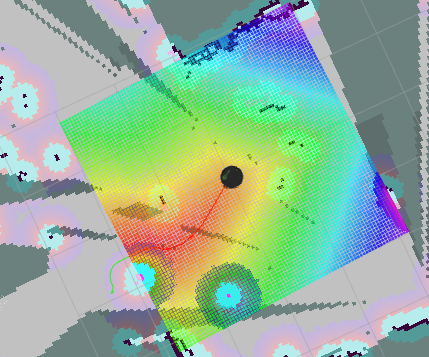
\includegraphics[width=0.5\textwidth]{figures/30cm.png}
    \caption{avoiding obstacle} 
    \label{fig:30cm} 
\end{figure}
\newpage

%
%
% Test 6
%
%

\section{Test 6}
The requirement, "The robot needs to be able to detect obstacles, with a minimum height 16 cm and a width of 3 cm, at a distance of up to 3.3 m", is tested by placing a wooden pole 4 m in front of the robot. Then by manual control, bringing the turtlebot closer to the object until the distance is 3.3 m.\\ 
\newline
First the host computer gets the commands:

1. \texttt{roscore}

2. \texttt{roslaunch\_bringup minimal.launch}

3. \texttt{roslaunch turtlebot\_navigation gmapping\_demo.launch}\\
On the user computer the commands is written in the terminal:

1. \texttt{roslaunch turtlebot\_rviz\_launchers view\_navigation.launch.}

2. \texttt{roslaunch turtlebot\_teleop keyboard\_teleop}\\
The program Rviz will open and by using the teleop it is possible to move the turtlebot towards the object. When the objects appears in rviz, a measurement will be made.

\subsection{Result}
The turtlebot detected the wooden pole within the 3.3 m distance.\\
Test 6 was successful and met the standards of the requirement.
%The turtlebot could not see the first object, which was a sign with a reflective surface. So the main object was tested instead, and this was a log without any reflective surfaces.
%The object would then appear at a 3.3 meters distance, which means this test was successful, and met the standards of the requirement.

%
%
% Test 7
%
%

\section{Test 7} 
The requirement, "The robot needs to be able to detect ledges at distances of 2 m or more", is tested by placing the turtlebot 2 m from the staircase at the test site, with its direction faced towards the staircase. Using the exploration node, the area of stairs will be marked and explored.\\ 
\newline
The host computer got the commands:

1. \texttt{roscore} 

2. \texttt{roslaunch turtlebot\_bringup minimal.launch}

3. \texttt{roslaunch turtlebot\_navigation gmapping\_demo.launch}\\
The user computer was given the commands in two different terminals:

1. \texttt{roslaunch turtlebot\_rviz\_launchers view\_navigation.launch}

2. \texttt{roslaunch turtlebot\_samples exploration.launch}\\
Using publish points, it will then explore the area chosen.
%To test this, we placed the robot 2 metres away from the lower staircase, with its direction faced towards the staircase.\\
%We then check the rviz map, if it shows whether there is a ledge or not, in the direction faced.

\subsection{Result}
The robot detected a "fall" in the map before 2 m, see figure \ref{fig:ledge}, but it did not stop before the cliff-sensor of the robot was activated at the very edge of the stairs.\\
Test 7 was successful and met the standards of the requirement.
\begin{figure}[h]
    \centering
    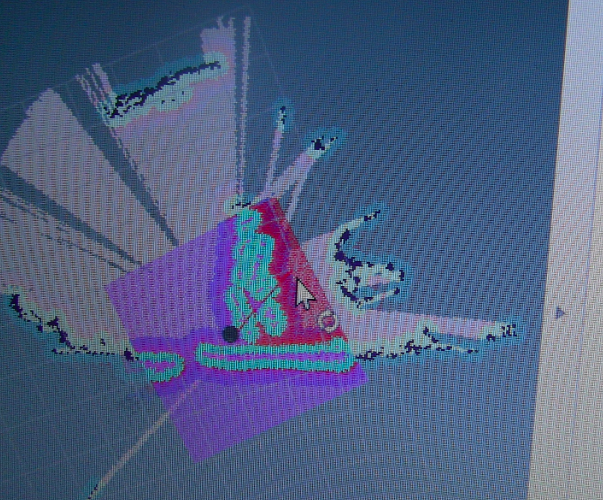
\includegraphics[width=0.5\textwidth]{figures/ledgePicture.png}
    \caption{Lower staircase ledge} 
    \label{fig:ledge} 
\end{figure}